% used inside TikZ, thus must be accessible to PlasTeX as well
\usepackage[dvipsnames]{xcolor}

% HTML from website SASS
\definecolor{brzdimeBlue}{HTML}{336699}
\definecolor{brzdimeOrange}{HTML}{ff9300}
\colorlet{brzdimeBlueBg}{brzdimeBlue!20}
\colorlet{brzdimeOrangeBg}{brzdimeOrange!20}
% semantic foreground
\colorlet{brzdimeAuto}{brzdimeBlue}
\colorlet{brzdimeSober}{brzdimeOrange}
% semantic background
\colorlet{brzdimeAutoBg}{brzdimeAuto!20}
\colorlet{brzdimeSoberBg}{brzdimeSober!20}


\newcommand*\cleartoleftpage{%
  \clearpage
  \ifodd\value{page}\thispagestyle{empty}\hbox{}\newpage\fi
}


\usepackage{tikz}
\usetikzlibrary{
	matrix,fit,shapes.callouts,shapes.arrows,shapes.misc,positioning,decorations.pathmorphing,arrows.meta,fpu,shapes.multipart,mindmap,arrows
}


% https://tex.stackexchange.com/a/72793
\tikzset{
	outlined arrow/.style args={#1 colored by #2 and #3}{
		-latex,
		line width=#1,color=#2,
		postaction={draw,-latex,color=#3,line width=(#1)/3,shorten <=(#1)/4,shorten >=4.5*(#1)/3}
	}
}

% https://tex.stackexchange.com/a/61362/6758
\tikzset{
	every fit/.append style=text badly centered,
}

% https://tex.stackexchange.com/a/8473/6758
\newcommand*\circled[1]{\tikz[baseline=(char.base)]{
    \node[shape=circle,draw,inner sep=2pt] (char) {#1};
}}

%\tikzset{
%  disable rounded corners for decorations/.style={
%    /pgf/every decoration/.style={
%      /tikz/sharp corners
%    },
%  }
%}

\tikzset{>=latex}

\tikzset{
	% custom asymetric columnns
	left column/.style args={below #1}{at=(#1.south),anchor=north east,shift=({-.5em,-1em})},
	right column/.style args={below #1}{at=(#1.south),anchor=north west,shift=({.5em,-1em})},
	narrower left column/.style args={below #1}{at=(#1.south),anchor=north east,shift=({-.5em-.15\linewidth,-1em})},
	wider right column/.style args={below #1}{at=(#1.south),anchor=north west,shift=({.5em-.15\linewidth,-1em})},
	% custom styles
	thought/.style={dashed,rounded corners,font=\itshape},
	action/.style={solid,sharp corners},
	% FIXME: why not 2\pgfkeysvalueof ??
	wider sober/.style={
		fill=brzdimeSoberBg,align=justify,dotted,rectangle split,rectangle split parts=2,sharp corners,
		text width=.65*(\linewidth-1em)-1*\pgfkeysvalueof{/pgf/inner xsep}-2*\pgflinewidth
	},
	sober/.style={fill=brzdimeSoberBg,align=justify,dotted,rectangle split,rectangle split parts=2,sharp corners},
	mindful/.style={fill=brzdimeSoberBg,align=center,dotted},
	narrower autopilot/.style={
		fill=brzdimeAutoBg,
		text width=.35*(\linewidth-1em)-1*\pgfkeysvalueof{/pgf/inner xsep}-2*\pgflinewidth
	},
	autopilot/.style={fill=brzdimeAutoBg,dashed},
	sober arrow/.style={outlined arrow={.5mm colored by black and brzdimeSoberBg}},
	wide sober arrow/.style={outlined arrow={1mm colored by black and brzdimeSoberBg}},
	autopilot arrow/.style={outlined arrow={.5mm colored by black and brzdimeAutoBg}},
	wide autopilot arrow/.style={outlined arrow={1mm colored by black and brzdimeAutoBg}},
}

\def\soberName#1{\textbf{#1} \nodepart{two} }

\def\mbrpset#1{\pgfkeys{/mbrp/.cd,#1}}
\pgfkeys{/mbrp/.is family,/mbrp,
	title1/.initial=\undefined,
	title2/.initial=\undefined,
	autopilot/.store in=\mbrpAutopilot,
	sober S/.initial={Pause and step out of automatic pilot mode.},
	sober O/.store in=\mbrpBrzdaR,
	sober O/.initial=\undefined,
	sober B/.initial={Take a few slow, mindful breaths in and out. Focus your attention on the breath.},
	sober E/.initial={Expand your awareness back to how you are feeling. Do your best to bring a sense of openness and acceptance to your experience.},
	sober R/.store in=\mbrpBrzdaA,
	sober R/.initial=\undefined,
	%
	title/.initial=\undefined,
	title/.store in=\mbrpTitle,
	toc title/.initial=\relax,
	toc title/.store in=\mbrpTocTitle,
	summary/.initial=\undefined,
	informal moments/.initial=\undefined,
	informal challenges/.initial=\undefined,
	informal activities/.initial=\undefined,
	formal/.initial=\undefined,
	practice sheets/.initial=\undefined
}

\newcommand{\mbrpSession}[1]{
	\bgroup
	\let\mbrpTocTitle\relax
	\mbrpset{#1}
	\cleardoublepage
	\addtocounter{section}{1}
	\setcounter{subsection}{0}
	\ifx\mbrpTocTitle\relax\let\mbrpTocTitle\mbrpTitle\fi
	\xdef\toct{\arabic{section}. \mbrpTocTitle}
	\sectionmark{\mbrpTocTitle}
	\addcontentsline{toc}{section}{\toct}
	\thispagestyle{start-session}
	\bgroup
		\null\vskip1cm
		\begin{tcolorbox}[
			skin=bicolor,
			boxrule=.4pt,
			coltitle=black,
			colbacktitle=brzdimeBlueBg,
			colback=white,
			parbox=false,
			adjusted title={\textbf{\Large\strut Session \arabic{section}}},
			% subtitle style={before={\vspace*{-1ex}}}
			%frame hidden,
		]
			\vskip1em
			{ \scshape\bfseries\Large\strut \mbrpTitle }
			\vskip1.5em
			\tcbsubtitle{{\large\strut \textbf{Key Concepts}}}
			\vskip.5em
			{\let\item\par \par\pgfkeysvalueof{/mbrp/summary}\par}
			\vskip.5em
		\end{tcolorbox}

		\clearpage

		\begin{tcolorbox}[
			skin=bicolor,
			boxrule=.4pt,
			%frame hidden,
			title={\strut Formal Practice},
			parbox=false,
			coltitle=black,
			colbacktitle=brzdimeOrangeBg,
			colback=white,
			fonttitle=\bfseries\large,
			% subtitle style={before={\vspace*{-1ex}}}
		]
			Do your best to listen to an audio-guided mindfulness exercise on a daily or semi-daily basis (4 to 6 days per week). Go to \href{https://PracticeMBRP.com}{PracticeMBRP.com} to access the exercises. Try to practice at the same time each day (such as before breakfast).

			We recommend focusing on these audio-guided exercises over the next few days/week:
				\begin{itemize*}
					\pgfkeysvalueof{/mbrp/formal}
				\end{itemize*}
			\medskip
			\tcbsubtitle{\strut On-the-Go Practice} % , za pochodu}
				\begin{description}
					\item[Mindful Moments:] \pgfkeysvalueof{/mbrp/informal moments}
					\item[Mindful Coping:]   \pgfkeysvalueof{/mbrp/informal challenges}
					\item[Mindful Activities:] \pgfkeysvalueof{/mbrp/informal activities}
				\end{description}
			\tcbsubtitle{\strut Handouts \normalPencilLeftDown}
				\begin{itemize*}
					\pgfkeysvalueof{/mbrp/practice sheets}
					\item My Practice Log.
				\end{itemize*}
				\medskip
		\end{tcolorbox}
	\egroup
	\clearpage
	\egroup
}


\newcommand{\soberSpace}[1]{
	\begin{adjustbox}{width=\linewidth,height=.9\textheight,keepaspectratio}
	\begin{tikzpicture}[
		every node/.style={
			align=center,
			text width=(\linewidth-1em)/2-2*\pgfkeysvalueof{/pgf/inner xsep}-2*\pgflinewidth,
			draw,
			rounded corners,
		},
		node distance=1em,
	]
	\mbrpset{#1}

	\node(top)[text width=.9\linewidth,text badly centered]{ \textsc{\pgfkeysvalueof{/mbrp/title1}} \\ \pgfkeysvalueof{/mbrp/title2} };
	\node(a0)[narrower autopilot, narrower left column=below top]{a0};
	\node(a0)[narrower autopilot,draw=none,narrower left column=below top]{$\downarrow${} \textsc{Autopilot} $\downarrow$};
	\draw[autopilot arrow] (top)--(a0);
	\foreach [var=\type,var=\content,count=\curr,remember=\curr as \prev (initially 0)] in \mbrpAutopilot {
		\node(a\curr) [narrower autopilot,\type,below=of a\prev]{\content};
		\draw[autopilot arrow] (a\prev.south)--(a\curr.north);
	}


	\node(b1)[wider sober,wider right column=below top]{\soberName{Stop.} \pgfkeysvalueof{/mbrp/sober S}};
	\node(b2)[wider sober,below=of b1]{\soberName{Observe.} Observe your experience without judgment: \begin{iitemize}\foreach\content in\mbrpBrzdaR{\item\content}\end{iitemize}};
	\node(b3)[wider sober,below=of b2]{\soberName{Breathe.} \pgfkeysvalueof{/mbrp/sober B}};
	\node(b4)[wider sober,below=of b3]{\soberName{Expand.} \pgfkeysvalueof{/mbrp/sober E}};
	\node(b5)[wider sober,below=of b4]{\soberName{Respond.} Respond with awareness. \begin{iitemize}\foreach\content in\mbrpBrzdaA{\item\content}\end{iitemize}};
	\begin{scope}
		\draw[sober arrow] (top) -- (b1);
		\draw[sober arrow] (b1) -- (b2);
		\draw[sober arrow] (b2) -- (b3);
		\draw[sober arrow] (b3) -- (b4);
		\draw[sober arrow] (b4) -- (b5);
	\end{scope}
	\end{tikzpicture}
	\end{adjustbox}
}

\newcommand{\soberSpaceEmpty}[1]{
	%\begin{adjustbox}{width=\linewidth,height=.85\textheight,keepaspectratio}
	\mbrpset{#1}
	\def\miniStrut{\rule[-.4ex]{0pt}{0pt}}
	\def\myslenkyPocityJednani{\leavevmode\lower.3ex\hbox{\vbox{\tiny\baselineskip=0pt\lineskip=-.3ex\hbox{thoughts}\hbox{feelings}\hbox{actions}}}}
	\def\teloPocityMysl{\leavevmode\lower.3ex\hbox{\vbox{\tiny\baselineskip=0pt\lineskip=-.3ex\hbox{body\miniStrut}\hbox{feelings\miniStrut}\hbox{mind\miniStrut}}}}
	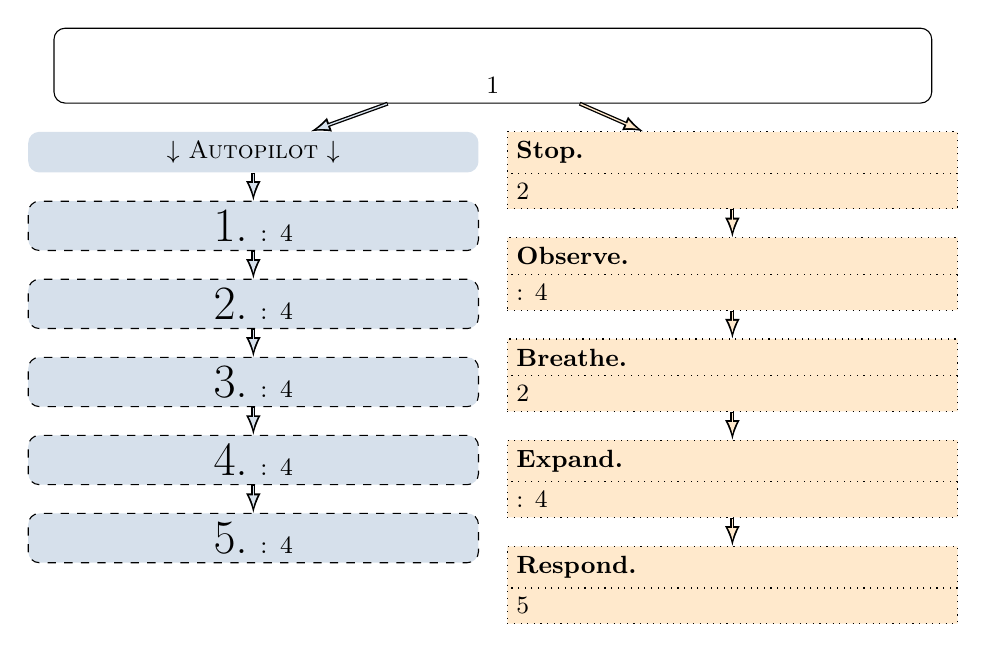
\begin{tikzpicture}[
		every node/.style={
			align=center,
			text width=(\linewidth-1em)/2-2*\pgfkeysvalueof{/pgf/inner xsep}-2*\pgflinewidth-4pt,
			% minimum width=(\linewidth-1em)/2, %-2*\pgfkeysvalueof{/pgf/inner xsep}-2*\pgflinewidth,
			draw,
			rounded corners,
			font=\small
		},
		node distance=1em,
	]
	\node(top)[text width=.9\linewidth]{\textsc{\pgfkeysvalueof{/mbrp/title1}} \\ \rule{0em}{5ex}\Blank{1}};
	\node(a0)[autopilot,draw=none,left column=below top]{$\downarrow${} \textsc{Autopilot} $\downarrow$};
	\draw[autopilot arrow] (top)--(a0);
	\foreach [var=\curr,remember=\curr as \prev (initially 0)] in {1,2,3,4,5} {
		\node(a\curr) [autopilot,below=of a\prev]{{\LARGE \curr.} \myslenkyPocityJednani: \Blank{4}};
		\draw[autopilot arrow] (a\prev.south)--(a\curr.north);
	}


	\node(b1)[sober,right column=below top]{\soberName{Stop.} \Blank{2}};
	\node(b2)[sober,below=of b1]{\soberName{Observe.} \teloPocityMysl: \Blank{4}};
	\node(b3)[sober,below=of b2]{\soberName{Breathe.} \Blank{2}};
	\node(b4)[sober,below=of b3]{\soberName{Expand.} \teloPocityMysl: \Blank{4}};
	\node(b5)[sober,below=of b4]{\soberName{Respond.} \Blank{5}};

	\begin{scope}
		\draw[sober arrow] (top) -- (b1);
		\draw[sober arrow] (b1) -- (b2);
		\draw[sober arrow] (b2) -- (b3);
		\draw[sober arrow] (b3) -- (b4);
		\draw[sober arrow] (b4) -- (b5);
	\end{scope}
	\end{tikzpicture}
	%\end{adjustbox}
}

\def\pageBRZDAown#1#2{
	% \clearpage\subsection*{#1 \normalPencilLeftDown}
	\vskip-1em #1{}
		How can you use the \textsc{Sober} space in the situation? For each step of the \text{Sober} write out what you would do/what you would notice in your own words. \par
	\vskip0pt minus1cm
	\soberSpaceEmpty{title1={#2}}
}



\def\pageGuesthouse{
	\clearpage
	\subsection{The Guest House Poem}
	% FROM https://tex.stackexchange.com/a/196934/6758
	\newlength{\saveleftmargini}
	\setlength{\saveleftmargini}{\leftmargini}
	\setlength{\leftmargini}{0em}
	\begin{verse}
		This being human is a guest house.\\
		Every morning a new arrival.

		A joy, a depression, a meanness,\\
		some momentary awareness comes\\\
		as an unexpected visitor.

		Welcome and entertain them all!\\
		Even if they are a crowd of sorrows,\\
		who sweep your house\\
		empty of its furniture,\\
		still, treat each guest honorably.\\
		They may be clearing you out\\
		for some new delight.

		The dark thought, the shame, the malice.\\
		meet them at the door and invite them in.

		Be grateful for whatever comes.\\
		Because each has been sent\\
		as a guide from beyond.
	\end{verse}
	\setlength{\leftmargini}{\saveleftmargini}
	\hskip.5\linewidth\emph{Rumi}
	% \vfill
}


\def\pageBRZDA{
	\subsection{\textsc{Sober} Space}
		The \textsc{Sober} Space is an \emph{on-the-go} mindfulness practice that you can do anywhere, anytime because it is brief, simple, and flexible.

		It can be used in a stressful situation, if you are upset, or when you are experiencing urges or impulses to engage in unwanted behavior. It can also be used when things are going well, when you are having fun, or any other time you want to more fully “show up” to appreciate the present moment. It can help you step out of “automatic pilot” and be more aware and mindful in your response. 
		\begin{itemize}
			\itemStop{S}{Stop.} Remember to stop or “pause” to do this exercise. This is the first step in stepping out of automatic pilot. 
			\itemStop{O}{Observe.} Observe what is going on in the moment, both around you and inside of you (body sensations, emotions, and thoughts). Try to observe with a sense of curiosity and nonjudgment. 
			\itemStop{B}{Breathe.} Notice the sensations of the breath in your body as you take a few slow breaths in and out. 
			\itemStop{E}{Expand.} Expand your awareness beyond just the breath to your whole body and then to the whole situation you are in.
			\itemStop{R}{Respond.} Respond to the situation with awareness, rather than reacting automatically. Recognize that you have choices for how to respond. Think about what you need and how you can take care of yourself. 
		\end{itemize}
	}

	\def\pagePracticeLog{
		%\par\vfill\pagebreak % this will acutally flush the previous page (unlike clearpage) and \newgeometry won't affect the previous page
		%\newgeometry{right=1cm,bottom=1cm} % top=1cm,left=1cm
		\practiceSheetTitle{My Practice Log}
		%\enlargethispage{5cm}
		\bgroup
			\def\myStrut{\rule{0pt}{\dimexpr(\pagewidth+5mm-8em-2cm-6em-3pt)/7}} % {.07\textheight}}
			\footnotesize
			%\noindent\kern-5mm
			\begin{adjustbox}{angle=90,Trim={10mm 50mm 0mm 5mm}}
			\begin{tblr}{
				width=\dimexpr\textheight+18mm\relax,
				colspec={X[l,1.3]|X[l,4]|X[l,4]|X[l,2]},
				%row{2}={font=\tiny}
			}
				{Date \\ Day } & {
					\textbf{Planned Practice} \\
					{\tiny Set aside time to listen to audio-guided exercise} \\
					Which practice? How long? 
				} & {
					\textbf{On-the-Go Practice:} \\
					\textbf{Mindful Moment}: took a random moment to pause/check-in \\
					\textbf{Mindful Coping}: Used \textsc{Sober} Space in challenging situation \\
					\textbf{Mindful Activity}: eating, walking, chores, being outside. \\
					What did you do? How many times?
				} & { Notes \\ Observations  } \\
				\hline \myStrut & \myStrut & \myStrut & \myStrut \\
				\hline \myStrut & \myStrut & \myStrut & \myStrut \\
				\hline \myStrut & \myStrut & \myStrut & \myStrut \\
				\hline \myStrut & \myStrut & \myStrut & \myStrut \\
				\hline \myStrut & \myStrut & \myStrut & \myStrut \\
				\hline \myStrut & \myStrut & \myStrut & \myStrut \\
				\hline \myStrut & \myStrut & \myStrut & \myStrut \\
			\end{tblr}
			\end{adjustbox}
		\egroup
		% \restoregeometry
	}



\def\pageBasicFeelings{
	\clearpage
	\subsection[Some Basic Feelings We All Have]{Some Basic Feelings We All Have\footnote{\href{https://www.nonviolentcommunication.com/learn-nonviolent-communication/feelings/}{https://www.nonviolentcommunication.com/learn-nonviolent-communication/feelings/}.}}
		\label{basic-feelings-we-all-have}
		Feel free to use the following list as a inspiration for expanding the vocabulary of feelings which you can recognize and name:
		\begin{multicols}{2}
		Feelings when needs “are” fulfilled:
		\begin{itemize*}
			\item Amazed
			\item Confident
			\item Energetic
			\item Glad
			\item Inspired
			\item Joyous
			\item Optimistic
			\item Relieved
			\item Surprised
			\item Touched
			\item Comfortable
			\item Eager
			\item Fulfilled
			\item Hopeful
			\item Intrigued
			\item Moved
			\item Proud
			\item Stimulated
			\item Thankful
		\end{itemize*}
		\columnbreak
		Feelings when needs “are not” fulfilled:
		\begin{itemize*}
			\item Angry
			\item Confused
			\item Disappointed
			\item Distressed
			\item Frustrated
			\item Hopeless
			\item Irritated
			\item Nervous
			\item Puzzled
			\item Sad
			\item Annoyed
			\item Concerned
			\item Discouraged
			\item Embarrassed
			\item Helpless
			\item Impatient
			\item Lonely
			\item Overwhelmed
			\item Reluctant
			\item Uncomfortable
		\end{itemize*}
		\end{multicols}
}

\def\pageBasicNeeds{
	\subsection[Some Basic Needs We All Have]{Some Basic Needs We All Have\footnote{\href{https://www.nonviolentcommunication.com/learn-nonviolent-communication/feelings/}{https://www.nonviolentcommunication.com/learn-nonviolent-communication/feelings/}.}}
		\label{basic-needs-we-all-have}
		\setstretch{.95}
		Feel free to use the following list as a inspiration for expanding the vocabulary of needs which you can recognize and name:
		\begin{multicols}{2}
			\begin{itemize*}
				\item Autonomy
					\begin{itemize*}
						\item Choosing dreams/goals/values
						\item Choosing plans for fulfilling one’s dreams, goals, values
					\end{itemize*}
				\item Celebration
					\begin{itemize*}
						\item Celebrate the creation of life and dreams fulfilled
						\item Celebrate losses: loved ones, dreams, etc. (mourning)
					\end{itemize*}
				\item Integrity
					\begin{itemize*}
						\item Authenticity
						\item Creativity
						\item Meaning
						\item Self-worth
					\end{itemize*}
				\item Interdependence
					\begin{itemize*}
						\item Acceptance
						\item Appreciation
						\item Closeness
						\item Community
						\item Consideration
						\item Contribute to the enrichment of life
						\item Emotional Safety
						\item Empathy
						\item Honesty (the empowering honesty that enables us to learn from our limitations)
						\item Love
						\item Reassurance
						\item Respect
						\item Support
						\item Trust
						\item Understanding
					\end{itemize*}
				\item Physical Nutrutrance
					\begin{itemize*}
						\item Air
						\item Food
						\item Movement, exercise
						\item Protection from life-threatening forms of life: viruses, bacteria, insects, predatory animals
						\item Rest
						\item Sexual expression
						\item Shelter
						\item Touch
						\item Water
					\end{itemize*}
				\item Play
					\begin{itemize*}
						\item Fun
						\item Laughter
					\end{itemize*}
				\item Spiritual Communion
					\begin{itemize*}
						\item Beauty
						\item Harmony
						\item Inspiration
						\item Order
						\item Peace
					\end{itemize*}
			\end{itemize*}
		\end{multicols}
}

